\input{../YKY-preamble.tex}
\setmainfont[BoldFont=Alibaba_Sans_Regular.otf,ItalicFont=Alibaba_Sans_Light_Italic.otf]{Alibaba_Sans_Light.otf}

\usepackage[backend=biber]{biblatex}
\bibliography{../AGI-book}

\usepackage[active,tightpage]{preview}		% for continuous page(s)
\renewcommand{\PreviewBorder}{0.5cm}
\renewcommand{\thempfootnote}{\arabic{mpfootnote}}

\usepackage[absolute,overlay]{textpos}		% for page number on upper left corner

\usepackage{color}
\usepackage{mathtools}
\usepackage[hyperfootnotes=false]{hyperref}

% \usepackage[backend=biber,style=numeric]{biblatex}
% \bibliography{../AGI-book}
% \renewcommand*{\bibfont}{\footnotesize}

\usetikzlibrary{shapes}
\usepackage[export]{adjustbox}				% ??
\usepackage{verbatim} % for comments
% \usepackage{newtxtext,newtxmath}	% Times New Roman font

% \titleformat{\subsection}[hang]{\bfseries\large\color{blue}}{}{0pt}{} 
% \numberwithin{equation}{subsection}

\newcommand{\underdash}[1]{%
	\tikz[baseline=(toUnderline.base)]{
		\node[inner sep=1pt,outer sep=10pt] (toUnderline) {#1};
		\draw[dashed] ([yshift=-0pt]toUnderline.south west) -- ([yshift=-0pt]toUnderline.south east);
	}%
}%

\newcommand\reduline{\bgroup\markoverwith{\textcolor{red}{\rule[-0.5ex]{2pt}{0.4pt}}}\ULon}

%\DeclareSymbolFont{symbolsC}{U}{txsyc}{m}{n}
%\DeclareMathSymbol{\strictif}{\mathrel}{symbolsC}{74}
\DeclareSymbolFont{AMSb}{U}{msb}{m}{n}
\DeclareSymbolFontAlphabet{\mathbb}{AMSb}
% \setmathfont{Latin Modern Math}
\DeclareMathOperator*{\argmin}{arg\,min}

% \usepackage[most]{tcolorbox}
\tcbset{on line, 
	boxsep=4pt, left=0pt,right=0pt,top=0pt,bottom=0pt,
	colframe=red,colback=pink,
	highlight math style={enhanced}
}
\newcommand{\atom}{\vcenter{\hbox{\tcbox{....}}}}

\let\oldtextbf\textbf
\renewcommand{\textbf}[1]{\textcolor{blue}{\oldtextbf{#1}}}

\newcommand{\logic}[1]{{\color{violet}{\textit{#1}}}}
\newcommand{\underconst}{\includegraphics[scale=0.5]{../2020/UnderConst.png}}
\newcommand{\KBsymbol}{\vcenter{\hbox{\includegraphics[scale=1]{../KB-symbol.png}}}}
\newcommand{\token}{\vcenter{\hbox{\includegraphics[scale=1]{token.png}}}}
\newcommand{\proposition}{\vcenter{\hbox{\includegraphics[scale=0.8]{proposition.png}}}}

\begin{document}

\begin{preview}

\cc{
\title{\vspace{-1.5cm} \bfseries\color{blue}{\LARGE AGI 大统一理论}}
}{
\title{\vspace{-1.5cm} \bfseries\color{blue}{\LARGE AGI Grand Unification}}
}

% \author{YKY} % Your name
\date{\vspace{-2cm}} % Date, can be changed to a custom date

\maketitle

\setcounter{section}{-1}
\newcounter{mypage}
\setcounter{mypage}{1}

% (1) Circled page number on upper left corner
\begin{textblock*}{5cm}(2.1cm,2.3cm) % {block width} (coords) 
{\color{red}{\large \textcircled{\small \themypage}}}
\addtocounter{mypage}{1}
\end{textblock*}

\begin{minipage}{\textwidth}
\setlength{\parskip}{0.4\baselineskip}

\section{综述}

\begin{itemize}

	\item 大统一理论是在 \textbf{强化学习} 的框架下进行的,这是以 Richard Sutton 为代表人物 提出的理论框架。 

	\item 在 强化学习里 最辣手的一个问题,就是如何 储存和计算 所有 \textbf{状态} 之上的 \textbf{概率分布}。 对 AGI 来说,状态 = 思维空间。 我们需要的是 所有可能的思维之上的概率分布,而这是 AGI 的一个硬性需求,无法避免。 由于思维空间是高维的向量空间,它上面的概率分布是一个庞大的 mathematical object,很难在计算机上表示。 如果用 神经网络 表示,则问题是如何对这个概率分布进行 \textbf{采样} (sampling), 在神经网络里,这是很困难的。

	\item \textbf{Hopfield 网络}的权重 定义了一个 能量地势 (energy landscape),它可以看成是一个 implicit 的 \textbf{概率分布}。 透过 Hopfield 网络的 learning,可以改变这个概率分布。 \reduline{但这需要修改 Hopfield 网络的算法,将 能量 诠释成 概率},而这正是 \textbf{Boltzmann machine},也称作 EBM (Energy-Based Models).

	\item 根据 ``Hopfield Network is All You Need'' 论文\footnote{感谢 Eric Zeng 给我推荐这篇论文。},现代 Hopfield 网络的 state update rule 跟 \textbf{Transformer} 重合\footnote{注意这是 state update rule 而不是 learning update rule.  前者 更改 Hopfield 网络的 激活 状态; 后者 更改 Hopfield 网络的权重/记忆。}。 换句话说,每执行一次 Transformer,就会趋向 Hopfield 的能量最低点。 

	\item Transformer 的 softmax 可以看成是 \textbf{大脑}中某种 ``winner-takes-all'' 机制。 从这个角度,可以类比大脑思考的机制,互相参考以获取更多灵感。
	
	\item 我最新的论文 提出,Transformer 具有 \textbf{逻辑结构},可以在逻辑基础上建立 AGI.

\end{itemize}


\end{minipage}
\end{preview}

\begin{preview}
\begin{minipage}{\textwidth}
\setlength{\parskip}{0.4\baselineskip}

\begin{textblock*}{20cm}(2.1cm,2cm) % {block width} (coords) 
	{\color{red}{\large \textcircled{\small \themypage}}}
	\hspace{8cm}
	\color{blue}{\footnotesize \cc{AGI 大统一理论}{AGI Unification}}
\end{textblock*}
\addtocounter{mypage}{1}
\vspace*{0.3cm} 

\section{Hopfield \cc{网络}{Networks}}

\cc{
Hopfield 网络是一种 特别简单的 fully-connected 神经网络,它具有 \textbf{associative memory} 的特性,可以凭部分 pattern 回忆整个 pattern:}{
Hopfield networks are a type of particularly simple, fully-connected neural networks, capable of \textbf{associative memory} retrieval:
}
\begin{equation}
\vcenter{\hbox{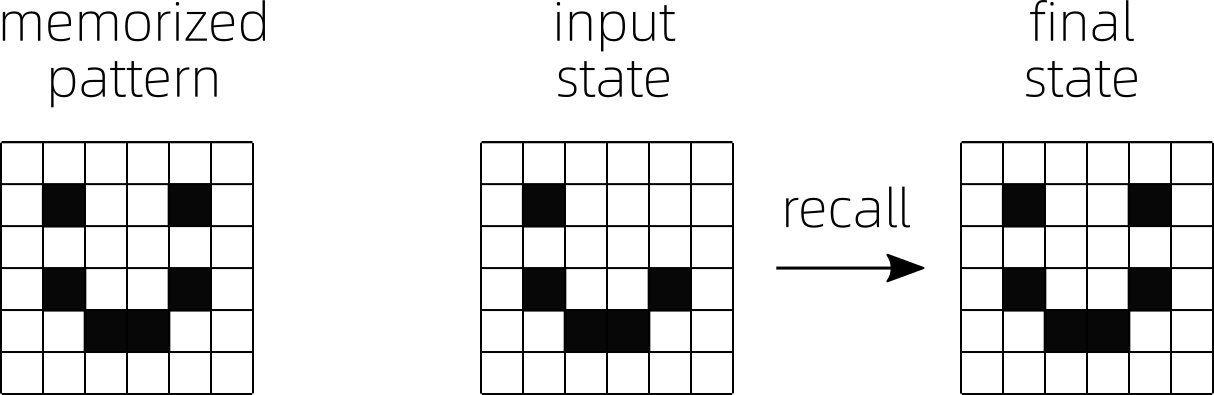
\includegraphics[scale=0.9]{Hopfield-network-example.png}}}
\label{fig:Hopfield-image-example}
\end{equation}
\cc{
记忆由神经元之间的 \textbf{连接权重} 决定,而这些权重定义了一个 \textbf{能量函数}。 Hopfield 网络就是统计物理学里面的 \textbf{Ising model} 应用到了神经网络上。 }{
Memory patterns are determined by connection weights of the network, which define an \textbf{energy function}.  The Hopfield network is actually the Ising model of statistical physics applied to neural networks.
}

\cc{
可以将一个 Hopfield 网络 铺平 画成这样:}{
One can flatten a Hopfield network and draw it like this:
}
\begin{equation}
\vcenter{\hbox{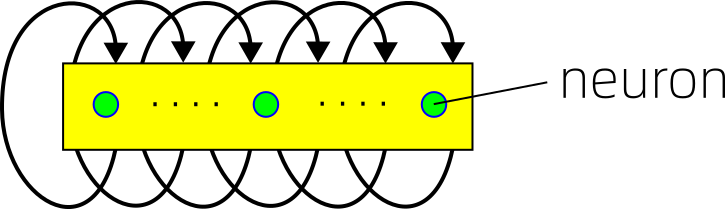
\includegraphics[scale=0.8]{Hopfield-network-1.png}}}
\label{fig:Hopfield-network}
\end{equation}
\cc{
注意它不是 feed-forward 网络,它的 输入 和 输出 在同一地方。}{
Note that it is not a feed-forward network;  its input and output neurons are the same.
}

\subsection{\cc{经典 Hopfield 网络}{Classical Hopfield Network}}

\cc{
我们的符号跟随 \textit{Hopfield Network is All You Need} [2021].}{
Our notation follows \textit{Hopfield Network is All You Need} [2021].
}

\cc{
$\vect{x}^i$ = 需要记忆的 \textbf{patterns} (有 $N$ 个), $x^i_{s}$ 是它的 $s$-th bit.}{
$\vect{x}^i$ = \textbf{memory patterns}.  There are $N$ of them, $x^i_{s}$ is the $s$-th bit of the $i$-th pattern.
}

\cc{
$\vect{X} = (\vect{x}^1, ... , \vect{x}^N)$ 是所有 patterns 的矩阵。}{
$\vect{X} = (\vect{x}^1, ... , \vect{x}^N)$ is the matrix containing all memory patterns.
}

\cc{
$\vect{\xi}$ = 网络的 \textbf{状态},$\xi_s$ = $s$-th 神经元 的 激活状态。}{
$\vect{\xi}$ = \textbf{state} of the Hopfield net, $\xi_s$ = activation state of the $s$-th neuron.
}

\cc{
\textbf{连接权重} between $s$-th and $t$-th neurons:}{
\textbf{Connection weight} between the $s$-th and $t$-th neurons:
}
\begin{equation}
\boxed{\mbox{Weights}} \quad T_{s,t} = \sum_i x^i_s x^i_t
\end{equation}
Refering to figure (\ref{fig:Hopfield-image-example}), the weights actually record the \textbf{co-activation} of pixel pairs.

\cc{
\textbf{总能量} (Hamiltonian):}{
Total energy (Hamiltonian):
}

\begin{equation}
\boxed{\mbox{Energy}} \quad E = -\frac{1}{2} \sum_s \sum_{t \neq s} \xi_s T_{s,t} \xi_t
\end{equation}

\subsection{\cc{Modern Hopfield 网络}{Modern Hopfield Network}}

\cc{
在经典 Hopfield 网络里,当 A 和 B 两个 patterns 太靠近的时候,它们会互相干扰,导致可以储存的 patterns 数量不大。  现代 Hopfield 网络 改变 Hamiltonian 能量函数,令干扰减弱,可以储存数量更多的 patterns:}{
In the classical Hopfield network, when two patterns A and B are too close together, they would interfere, so the storage capacity is limited.  Modern Hopfield networks modify the energy function such that interference is reduced, resulting in greater storage capacity: 
}

\begin{equation}
\vcenter{\hbox{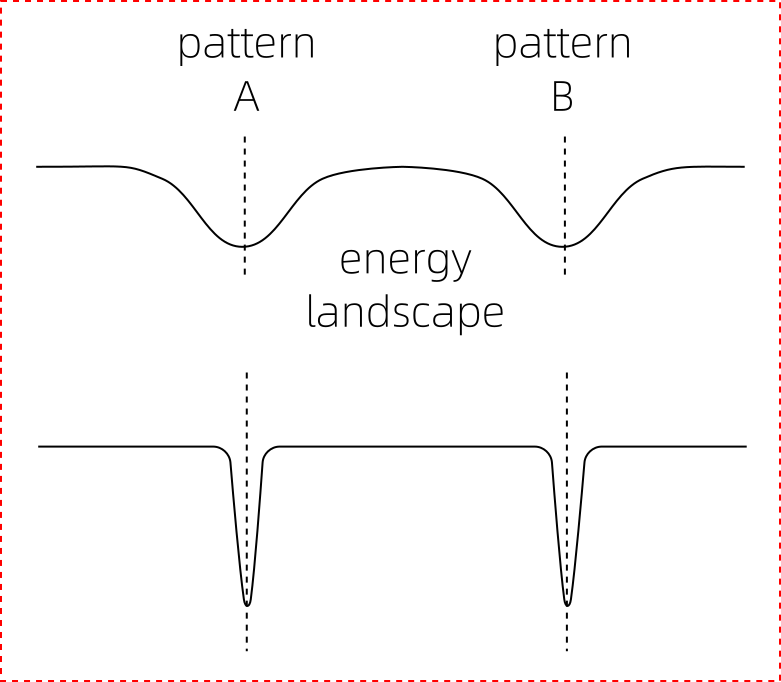
\includegraphics[scale=0.7]{modern-Hopfield-network-energy-landscape.png}}}
\end{equation}

\cc{
\textbf{新的能量}函数:}{
The \textbf{new energy function}:
}
\begin{equation}
\boxed{\mbox{New Energy}} \quad E = - \sum_i F( \vect{\xi}^T \vect{x}^i )
\end{equation}
\cc{注:}{Note: } $ \displaystyle \vect{\xi}^T \vect{x}^i = \sum_s \xi_s x^i_s$ , \; $F$ = interaction function.

\cc{
[Demircigil et al 2017] 提出 $F$ 用 exponential 函数。}{
[Demircigil et al 2017] proposes to use the exponential function for $F$.
}

\textbf{State update rule}:
\begin{equation}
\vect{\xi}^{\mbox{new}} = \vect{X} \; \mbox{softmax}(\beta \vect{X}^T \vect{\xi})
\end{equation}
This corresponds to the update rule of the conventional Transformer:
\begin{equation}
	\vect{Z} = \mbox{softmax} \left( \frac{1}{\sqrt{d_k}} \vect{Q} \, \vect{K}^T \right) \vect{V}
\end{equation}

\subsection{Hopfield-Transformer 对应}

\textbf{传统 Transformer}'s state update rule:
\begin{equation}
\vect{Z} = \mbox{softmax} \left( \frac{1}{\sqrt{d_k}} \vect{Q} \, \vect{K}^T \right) \vect{V}
\end{equation}

\textbf{Modern Hopfield network}'s state update rule:
\begin{equation}
\vect{Z} = \mbox{softmax} \left( \beta \vect{\hat{R}} \vect{\hat{Y}}^T \right) \vect{\hat{Y}}^T
\end{equation}
这里 $\vect{\hat{R}}, \vect{\hat{Y}}, \vect{\hat{X}}$ 是 $\vect{R}, \vect{Y}, \vect{X}$ 分别乘上了适当的 $\vect{W}$'s 矩阵,但为了数式的简洁,使用了代号。

Query patterns = $\vect{R} = (\vect{r}_1, ... , \vect{r}_M)$ 是网络的\textbf{状态}。 之所以有 $M$ 个状态,是因为他们将 Transformer 的 $M$ 个输入 \textbf{摊开}来,才构成一个大的 Hopfield 网。 \reduline{不这样做根本无法将 Hopfield 网和 Transformer 等同起来}。

$\vect{Y}$ 就是 Hopfield 记忆里的 patterns,它们担任 Transformer 里 \textbf{keys} 的角色。

在 Self-Attention 里,$\vect{R} = \vect{Y}$.

跟图 (\ref{fig:Hopfield-network}) 比较,这个是 受 Transformer 结构 约束的 Hopfield 网络:
\begin{equation}
\vcenter{\hbox{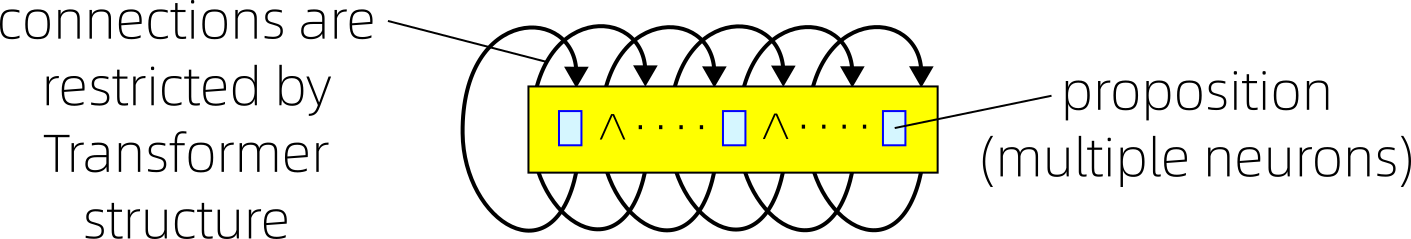
\includegraphics[scale=0.8]{Hopfield-network-as-Transformer.png}}}
\end{equation}

\end{minipage}
\end{preview}

\begin{preview}
\begin{minipage}{\textwidth}
\setlength{\parskip}{0.4\baselineskip}

\begin{textblock*}{20cm}(2.1cm,2cm) % {block width} (coords) 
	{\color{red}{\large \textcircled{\small \themypage}}}
	\hspace{8cm}
	\color{blue}{\footnotesize \cc{AGI 大统一理论}{AGI Unification}}
\end{textblock*}
\addtocounter{mypage}{1}
\vspace*{0.3cm} 

\section{Boltzmann 机}

注意: 以下是 Boltzmann machine 跟 \textbf{经典} Hopfield network 的对应。

Let $O = (O_1, ..., O_n)$ be the \textbf{state vector}.

$W = \{ W_{s,t} \}$ are connection \textbf{weights}.

\textbf{State update rule}:  $i$-th unit is set to 1 with probability
\begin{equation}
\frac{1}{1 + e^{- S_i / T}}
\end{equation}
where $T$ is a temperature.

如果用以上的 update rule,则 Hopfield 能量 变成 \textbf{概率分布}:
\begin{equation}
P(O) = P(O|W) = \frac{e^{-\mathcal{E}(O)/T}}{Z} \quad \boxed{\mbox{Boltzmann distribution}}
\end{equation}
where partition function $\displaystyle Z = \sum_U e^{-\mathcal{E}(U)/T} $

{\color{red}TO-DO:} \reduline{求出 现代版的 Hopfield network 的 Boltzmann state update rule}.


{\color{red}TO-DO:} \reduline{求出 Hopfield-Boltzmann machine 的 \textbf{learning} update rule}.  但它似乎是根据 \textbf{记忆} 而 update ??

\end{minipage}
\end{preview}

\begin{preview}
\begin{minipage}{\textwidth}
\setlength{\parskip}{0.4\baselineskip}

\begin{textblock*}{20cm}(2.1cm,2cm) % {block width} (coords) 
	{\color{red}{\large \textcircled{\small \themypage}}}
	\hspace{8cm}
	\color{blue}{\footnotesize \cc{AGI 大统一理论}{AGI Unification}}
\end{textblock*}
\addtocounter{mypage}{1}
\vspace*{0.3cm} 

\section{与强化学习 结合}

\subsection{LLM 内部很可能存在冗余}

LLM (大型语言模型) 是根据 自回归 (auto-regression, 强迫模型的输出跟输入一样) 的原理训练。 在这种模式下,Transformer 用大约一半的资源,将输入句子转化成一个 \reduline{具有高度抽象语义的 内在表示}。 它的后半部 利用这个抽象表示 去预测掩盖了的词语:
\begin{equation}
\vcenter{\hbox{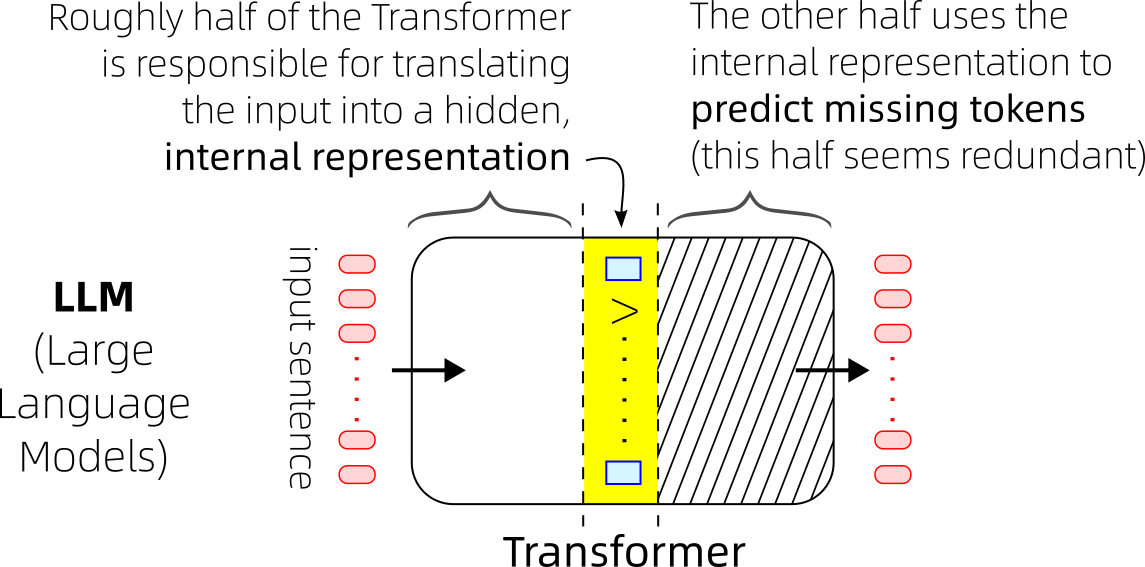
\includegraphics[scale=1]{redundancy-in-LLM-1.png}}}
\end{equation}
在一个智能系统里面,其实我们最需要的是 中间的那个 hidden representation,用来做「下游」的工作,但不一定是预测词语,所以后半部对智能系统来说,构成了一种\textbf{冗余}。

有两个做法: 一是接受这个冗余,继续将整个 AGI 系统做出来。 二是改变系统架构,重新训练一个更合乎直观的模型。

个人认为 强化学习 模型 更为直观,可以省却很多理解上的「拐弯抹角」,令 AGI 的设计更清晰:
\begin{equation}
\vcenter{\hbox{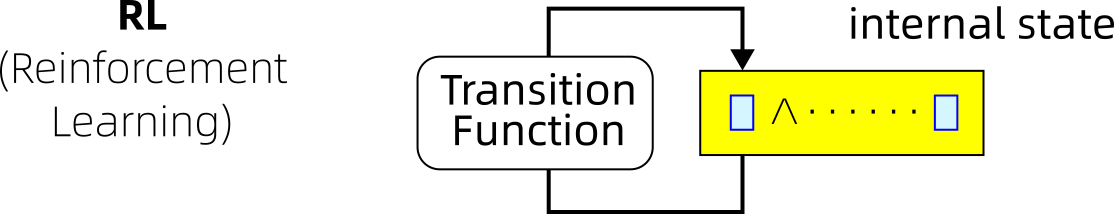
\includegraphics[scale=1]{redundancy-in-LLM-2.png}}}
\end{equation}
这个 transition function 就是一个类似 Transformer 的函数。

\subsection[Transformer]{Transformer $\rightarrow$ Hopfield $\rightarrow$ Boltzmann}

在强化学习里,系统需要 \textbf{储存} 并 \textbf{学习} 一个分布在所有状态或动作(包括 思维动作,即「思维空间」)之上的 \textbf{概率分布}。 由于思维空间是一个庞大的 高维向量空间,在计算机上很难处理。 (数学家们很轻松就写下这种空间,但我们必需考虑实践的可行性。 有人打趣说:「计算机学家就是赶时间的数学家」)

不能简单地用 Transformer 输出这个 概率分布。 目前习惯是,Transformer 输出的 token,会乘上一个矩阵,让输出转换成一支很长的向量,它代表 词典里每个词的概率分布。 但这个 trick 转到 思维空间上就不管用了,因为将所有可能的思维枚举出来 不切实际。

于是我们想到一个办法就是,用「隐式」的方法表示这个概率分布。 关键是一篇名为 “\textit{Hopfield Network is All You Need}” 的论文。 Hochreiter et al 论证,Transformer 是 Hopfield 网络的一个特例。

Hopfield 网络的能量函数可以转变为 概率,那就是 Boltzmann machine.  这个东西在深度学习里占有举足轻重的地位; Hinton、Bengio、LeCun 等人 都深入地研究过它,特别是因为它适用于 强化学习。 它也叫作 EBM (energy-based models).

Transformer 可以轻易地转变为 Hopfield 网络,然后变成 EBM.  那么,根据强化学习的 Bellman 方程,必然可以找到它的 learning update rule, 于是可以建立 AGI 的最基本模型。

这里还有一点细节需要想明白: 在 RL 的「状态」里面有很多逻辑命题,它们互相激活,导致下一个结论命题的出现。 这情况跟大脑里的 ``areas'' 互相激活 很相似。 或许大脑 可以给我们一些启发,如何更有效率地组织 大量 神经元之间的连接?
\begin{equation}
\vcenter{\hbox{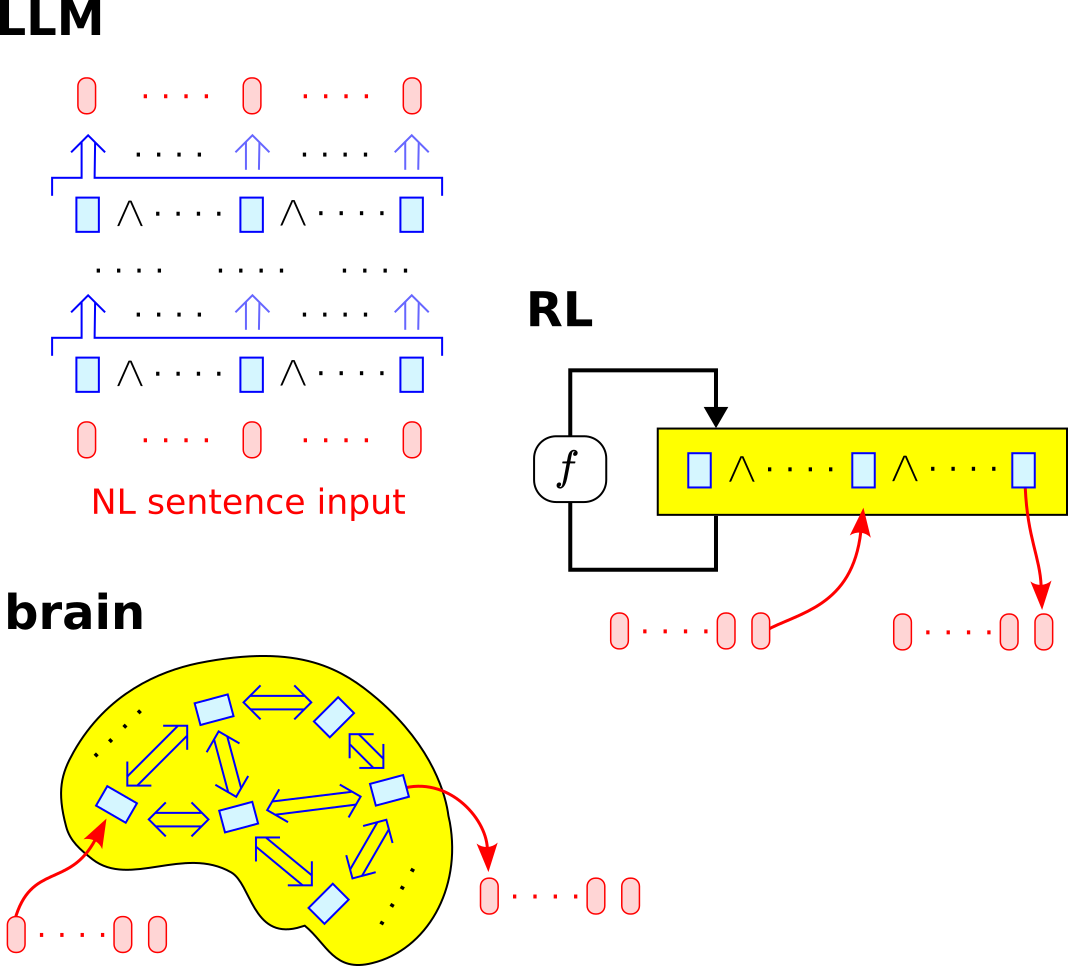
\includegraphics[scale=1]{LLM-vs-RL-vs-brain.png}}}
\end{equation}

\end{minipage}
\end{preview}

\begin{preview}
\begin{minipage}{\textwidth}
\setlength{\parskip}{0.4\baselineskip}

\begin{textblock*}{20cm}(2.1cm,2cm) % {block width} (coords) 
	{\color{red}{\large \textcircled{\small \themypage}}}
	\hspace{8cm}
	\color{blue}{\footnotesize \cc{AGI 大统一理论}{AGI Unification}}
\end{textblock*}
\addtocounter{mypage}{1}
\vspace*{0.3cm} 

\subsection{结合 Transformer + RL : Road Map}

如果我没理解错,Hopfield 网络 是 fully-connected, 可以这样表示:
\begin{equation}
	\vcenter{\hbox{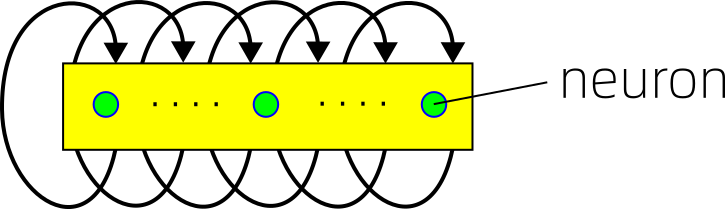
\includegraphics[scale=0.8]{Hopfield-network-1.png}}}
	\label{fig:1-layer-Hopfield-net}
\end{equation}

\subsubsection{第1步}
根据《Hopfield Network Is All You Need》,图(\ref{fig:1-layer-Hopfield-net}) 代表 一层的 Transformer 的 forward inference(但在 Hopfield 网络里,输入和输出的神经元是同一组):
\begin{equation}
	\vcenter{\hbox{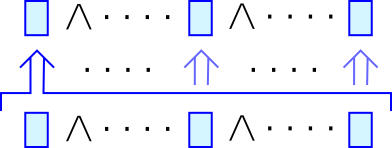
\includegraphics[scale=1]{1-layer-of-Transformer.png}}}
\end{equation}

\subsubsection{第2步}
我们希望 将 Hopfield $\rightarrow$ Boltzmann,让输出符合 概率分布。 但 Boltzmann machine 一般来说是 intractable 的,需要 restricted Boltzmann machine, 也就是一个 bipartite graph,这个 结构 让概率分布函数可以 factorize:
\begin{equation}
\vcenter{\hbox{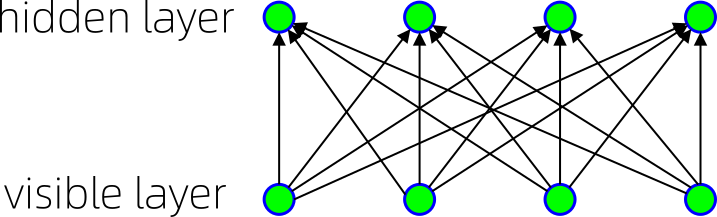
\includegraphics[scale=1]{restricted-Boltzmann-machine.png}}}
\label{fig:Boltzmann-machine}
\end{equation}
换句话说,图(\ref{fig:Boltzmann-machine}) 是 \textbf{概率化}了的 一层 Transformer。

\subsubsection{第3步}
然后,我们可以将 Boltzmann machine 叠起来,这类似于 传统的多层 Transformer,但是 概率化了:
\begin{equation}
\vcenter{\hbox{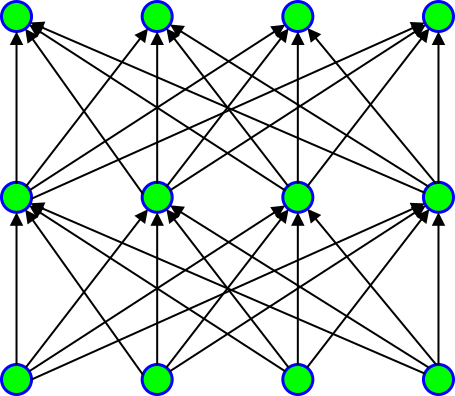
\includegraphics[scale=1]{multi-layer-Boltzmann-machine.png}}}
\label{fig:multi-layer-Boltzmann}
\end{equation}
到这一步以后,可以直接将这个网络嵌入 强化学习里,造成最简单的 AGI 模型。

\subsubsection{第4步}
(这步非必需,但可以作为参考,获得灵感)

图(\ref{fig:multi-layer-Boltzmann}) 有点类似大脑的 ``areas'' 结构:
\begin{equation}
\vcenter{\hbox{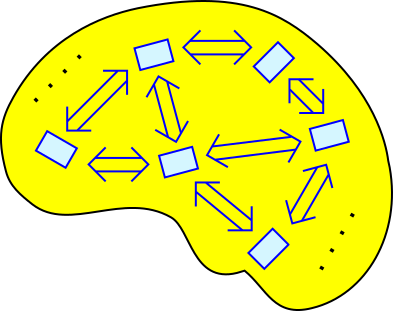
\includegraphics[scale=1]{brain-areas-structure.png}}}
\end{equation}
但不同于 图(\ref{fig:multi-layer-Boltzmann}) 的是,大脑 areas 之间的连接是 \textbf{双向}的。 但我们可以根据这一点启发,设计更有效率的 AGI 网络结构: 分成很多个 areas,areas 之间以 Transformer 连接。 新的 Transformer 或许可以是 双向的,但细节未弄清楚。

\end{minipage}
\end{preview}

\begin{preview}
\begin{minipage}{\textwidth}
\setlength{\parskip}{0.4\baselineskip}

\begin{textblock*}{20cm}(2.1cm,2cm) % {block width} (coords) 
	{\color{red}{\large \textcircled{\small \themypage}}}
	\hspace{8cm}
	\color{blue}{\footnotesize \cc{AGI 大统一理论}{AGI Unification}}
\end{textblock*}
\addtocounter{mypage}{1}
\vspace*{0.3cm} 

\subsection{RL update rule}

首先,\textbf{Deep Q Learning} (DQN) 的问题是它无法处理 连续的 action space(例如高维向量空间):
\begin{equation}
\vcenter{\hbox{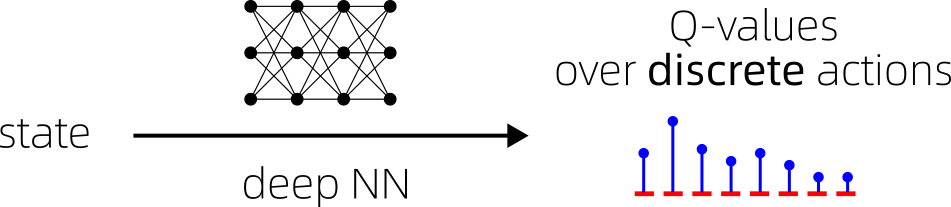
\includegraphics[scale=1]{deep-Q-learning.png}}}
\label{fig:DQN}
\end{equation}
所谓 Q-value 就是 $Q(s,a) =$ 在状态 $s$ 做动作 $a$ 的\textbf{价值}。 大家想想: 如果状态 $s$ 包含所有可能的思维状态,动作 $a$ 包含所有可能的思维动作,则 $Q(s,a)$ 的讯息就包含了一个智能系统的所有智慧!

(s,a) 是连续空间 这个问题可以用 \textbf{Energy-Based Model} (EBM) 解决,最早提出的似乎是 Hinton \& Sallans 2004 \cite{Sallans2004}, 而在那篇论文里,他们正正是为了解决 RL 问题\footnote{大家可参看《Quantum Enhancements for Deep Reinforcement Learning in Large Spaces》 [2021],此文的目标虽然是 量子计算,但它考察了 deep RL 的最新研究。}。 中心思想就是 \reduline{用 free energy\footnote{所谓 free energy 是指,在 Hopfield 或 Boltzmann 模型里,有 visible ($v_i$) 和 hidden ($h_i$) 神经元之分。 Energy $E$ 的表达式包含 $v_i$ 和 $h_i$.  Free energy 是 $E$ 对 $h_i$ 的求和,即 marginalization: $F(v) = \sum_{h} E(v,h)$.} $F$ 近似 Q-value}: $ Q(s,a) \approx -F(s,a) $.

强化学习 的 \textbf{Bellman update} 根据 状态 $s$ 的奖励 $R(s,a)$ 更新某价值函数, 例如我比较熟悉的 Q-Learning 的 temporal difference update:
\begin{equation}
% Q(s,a) \mathrel{+}= \eta \left[ R + \gamma \Delta Q \right]
Q(s,a) \mathrel{+}= \eta \left[ R(s,a) + \gamma \max_{a'} Q'(s',a') - Q(s,a) \right]
\end{equation}
( $\eta$ = learning rate, $\gamma$ = discount factor, $s$ = state, $a$ = action )\\
$Q$ 就是系统选择某行动的预期价值,系统(带有随机性地)选择 $Q$ 最大的那些动作。 这跟 Hopfield 或 Boltzmann 模型 里面的 状态转移 $s \rightarrow s'$ 的概率 或能量 $F$ 是异曲同工的。 

$Q$ 的 update rule 基本上就是 Hopfield 或 Boltzmann 模型的权重的 update rule.  这些初步工作已经被 Hinton \& Sallans 做了。 但这个 na\"{i}ve 的做法 可能不够计算效率,它甚至丧失了 back-prop,我们目前最强的武器!

(没有受限的)Boltzmann machine 只是一块扁平的东西:
\begin{equation}
\vcenter{\hbox{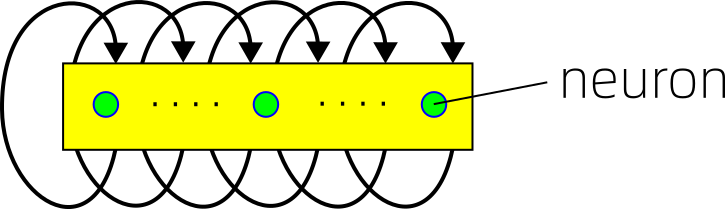
\includegraphics[scale=0.8]{Hopfield-network-1.png}}}
\end{equation}
对比于 图(\ref{fig:DQN}) 它缺少了「深度」,虽然 强化学习 的 loop 也可以看成是一种深度,但它跟 back-prop 好像不一样。 这样会不会丧失了深度学习的优势呢? 必需详细分析.....

有某些问题: \\
1. Hopfield / Boltzmann spin 出了 set of next propositions. \\
2. 想知道这些 propositions 的 $P(x_i | \vect{X})$, 但似乎不易。 \\
3. 

\printbibliography

\end{minipage}
\end{preview}

\begin{preview}
\begin{minipage}{\textwidth}
\setlength{\parskip}{0.4\baselineskip}

\begin{textblock*}{20cm}(2.1cm,2cm) % {block width} (coords) 
	{\color{red}{\large \textcircled{\small \themypage}}}
	\hspace{8cm}
	\color{blue}{\footnotesize \cc{AGI 大统一理论}{AGI Unification}}
\end{textblock*}
\addtocounter{mypage}{1}
\vspace*{0.3cm} 

\section{Personal Notes}

于是 Ngiam \textit{et al} 2011(在 Andrew Ng 为导师下)提出了 \textbf{Deep Energy Models} (DEMs).

下图中,我们比较 LLM, RL 和 大脑。 它们的\textbf{状态} 有什么对应关系? 
\begin{equation}
\vcenter{\hbox{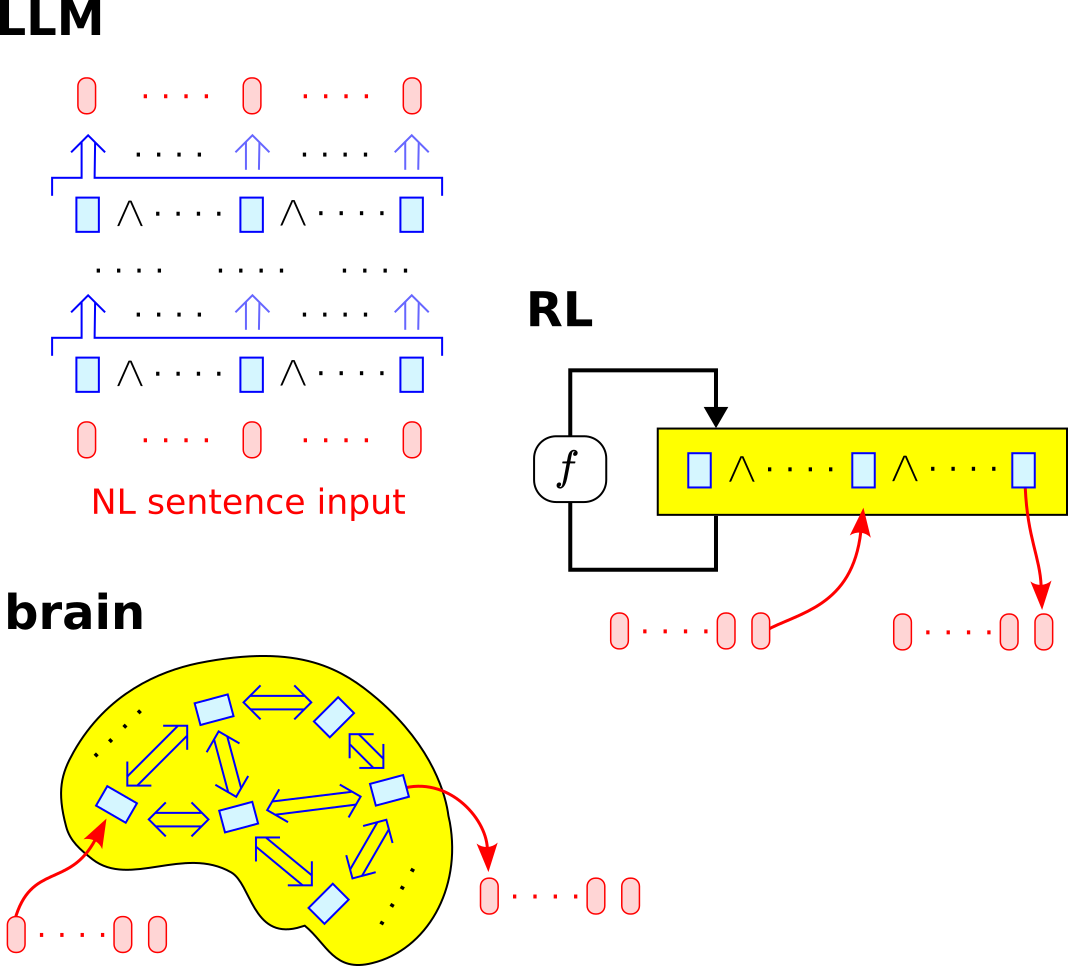
\includegraphics[scale=1]{LLM-vs-RL-vs-brain.png}}}
\end{equation}

从 model-based RL 的角度看(例如 PILCO),需要 预测世界。 但这不包括预测自己的思想。 但基于感觉资料的思想 包括对世界的预测。 模型就是对世界的思想。 究竟 model-based 跟 model-free 有什么分别?  对 世界的预测 帮助 寻找最佳的对策。 但我说 对世界的预测 是 sensory-based inference 而已。  

在状态之中 某些命题 update,但其他命题 可以不变。 

RL 里面,weights 决定 next state,utility 决定 next state,weights 决定 utility = energy = probability distribution over next states.  但 current state 的 utility value 似乎很难获得?  

State 跟 action 的分别,似乎就是 新命题 跟 命题集合 的分别。 

在大脑中,命题似乎有 位置的固定性。 

\underconst \quad 这部分暂时仍未想清楚....

\section{大脑}

\end{minipage}
\end{preview}

\end{document}
